% ---- pg-054 （书页 42） ----
其次,由 $\bm{x}'\bm{x} = 1^2 + 3^2 + 2^2 = 14$，$\bm{y}'\bm{y} = (-2)^2 + 1^2 + (-1)^2 = 6$,以及 $\bm{x}'\bm{y} = 1 \times (-2) + 3 \times 1 + 2 \times (-1) = -1$,有

\[
L_x = \sqrt{\bm{x}'\bm{x}} = \sqrt{14} = 3.742 \qquad L_y = \sqrt{\bm{y}'\bm{y}} = \sqrt{6} = 2.449
\]

和

\[
\cos(\theta) = \frac{\bm{x}'\bm{y}}{L_xL_y} = \frac{-1}{3.742 \times 2.449} = -0.109
\]

于是 $\theta = 96.3^\circ$.最后

\[
L_{3x} = \sqrt{3^2 + 9^2 + 6^2} = \sqrt{126}, \quad 3L_x = 3\sqrt{14} = \sqrt{126}
\]

可见 $L_{3x} = 3L_x$.

一对同维向量 $\bm{x}$ 和 $\bm{y}$,如果存在两个不全为零的常数 $c_1$ 和 $c_2$,满足

\phantomsection\label{eq:2-7}
\begin{equation}
c_1\bm{x} + c_2\bm{y} = \bm{0} \tag{2-7}
\end{equation}

就说这对向量线性相关.一组向量 $\bm{x}_1, \bm{x}_2, \cdots, \bm{x}_k$,如果存在不全为零的常数 $c_1, c_2, \cdots, c_k$,使得

\[
c_1\bm{x}_1 + c_2\bm{x}_2 + \cdots + c_k\bm{x}_k = \bm{0}
\]

就说这组向量线性相关.

线性相关意味着:这组向量中至少有一个向量能写成其余向量的线性组合.如果几个同维向量并不线性相关,就说它们线性无关.

\mvbold{例 2.2} （识别线性无关向量）

考虑向量组

\[
\bm{x}_1 = \begin{bmatrix} 1 \\ 2 \\ 1 \end{bmatrix} \qquad \bm{x}_2 = \begin{bmatrix} 1 \\ 0 \\ -1 \end{bmatrix} \qquad \bm{x}_3 = \begin{bmatrix} 1 \\ -2 \\ 1 \end{bmatrix}
\]

令

\[
c_1\bm{x}_1 + c_2\bm{x}_2 + c_3\bm{x}_3 = \bm{0}
\]

可推出

\[
c_1 + c_2 + c_3 = 0
\]
\[
2c_1 \qquad - 2c_3 = 0
\]
\[
c_1 - c_2 + c_3 = 0
\]

有唯一解 $c_1 = c_2 = c_3 = 0$.由于找不到不全为零的常数 $c_1$,$c_2$ 和 $c_3$,使得 $c_1\bm{x}_1 + c_2\bm{x}_2 + c_3\bm{x}_3 = \bm{0}$,因而向量 $\bm{x}_1$,$\bm{x}_2$ 和 $\bm{x}_3$ 线性无关.

向量 $\bm{x}$ 在向量 $\bm{y}$ 上的投影(或影子)为

\phantomsection\label{eq:2-8}
\begin{equation}
\bm{x} \text{ 在 } \bm{y} \text{ 上的投影} = \left(\frac{\bm{x}'\bm{y}}{\bm{y}'\bm{y}}\right)\bm{y} = \left(\frac{\bm{x}'\bm{y}}{L_y}\right)\frac{1}{L_y}\bm{y} \tag{2-8}
\end{equation}

其中向量 $L_y^{-1}\bm{y}$ 的长度为 1.投影的长度为

\phantomsection\label{eq:2-9}
\begin{equation}
\text{投影的长度} = \left| \frac{\bm{x}'\bm{y}}{L_y} \right| = L_x\left| \frac{\bm{x}'\bm{y}}{L_xL_y} \right| = L_x| \cos(\theta) | \tag{2-9}
\end{equation}

其中 $\theta$ 是 $\bm{x}$ 与 $\bm{y}$ 间的夹角(见\hyperref[fig:2.5]{图 2.5}).

\begin{mvfigure}
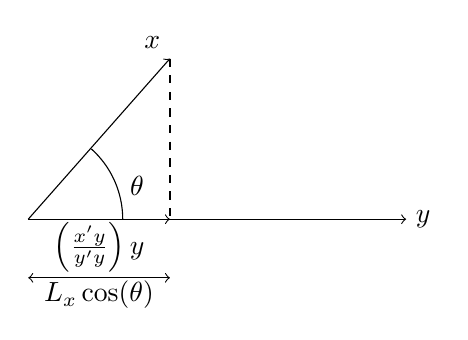
\begin{tikzpicture}[scale=1.2]
\draw[->] (0,0) -- (4.0,0) node[right] {$\bm{y}$};
\draw[->] (0,0) -- (1.5,1.7) node[above left] {$\bm{x}$};
\draw[dashed] (1.5,1.7) -- (1.5,0);
\draw[->] (0,0) -- (1.5,0);
\node[below,inner sep=1pt] at (0.75,0) {$\left(\frac{\bm{x}'\bm{y}}{\bm{y}'\bm{y}}\right)\bm{y}$};
\draw (1.0,0) arc (0:48:1.0);
\node at (1.15,0.35) {$\theta$};
\draw[<->] (0,-0.62) -- (1.5,-0.62);
\node[below,inner sep=1pt] at (0.75,-0.62) {$L_x\cos(\theta)$};
\end{tikzpicture}
\phantomsection\label{fig:2.5}\mvcap{图 2.5\quad $\bm{x}$ 在 $\bm{y}$ 上的投影}
\end{mvfigure}

\mvsub{矩阵}

由实数组成的任何矩形数表称为矩阵.我们将一个 $n$ 行 $p$ 列的任意数表示成
